\section{\name Prototype Overview}
\label{sec:prototype}

In this section we provide an overview of our \name prototype implementation. Due to space constrains full implementation details are given in Appendix~\ref{appendix:implementation}.

\begin{figure}[t]
    \begin{center}
        \begin{subfigure}{0.4\textwidth}
        \centering
            %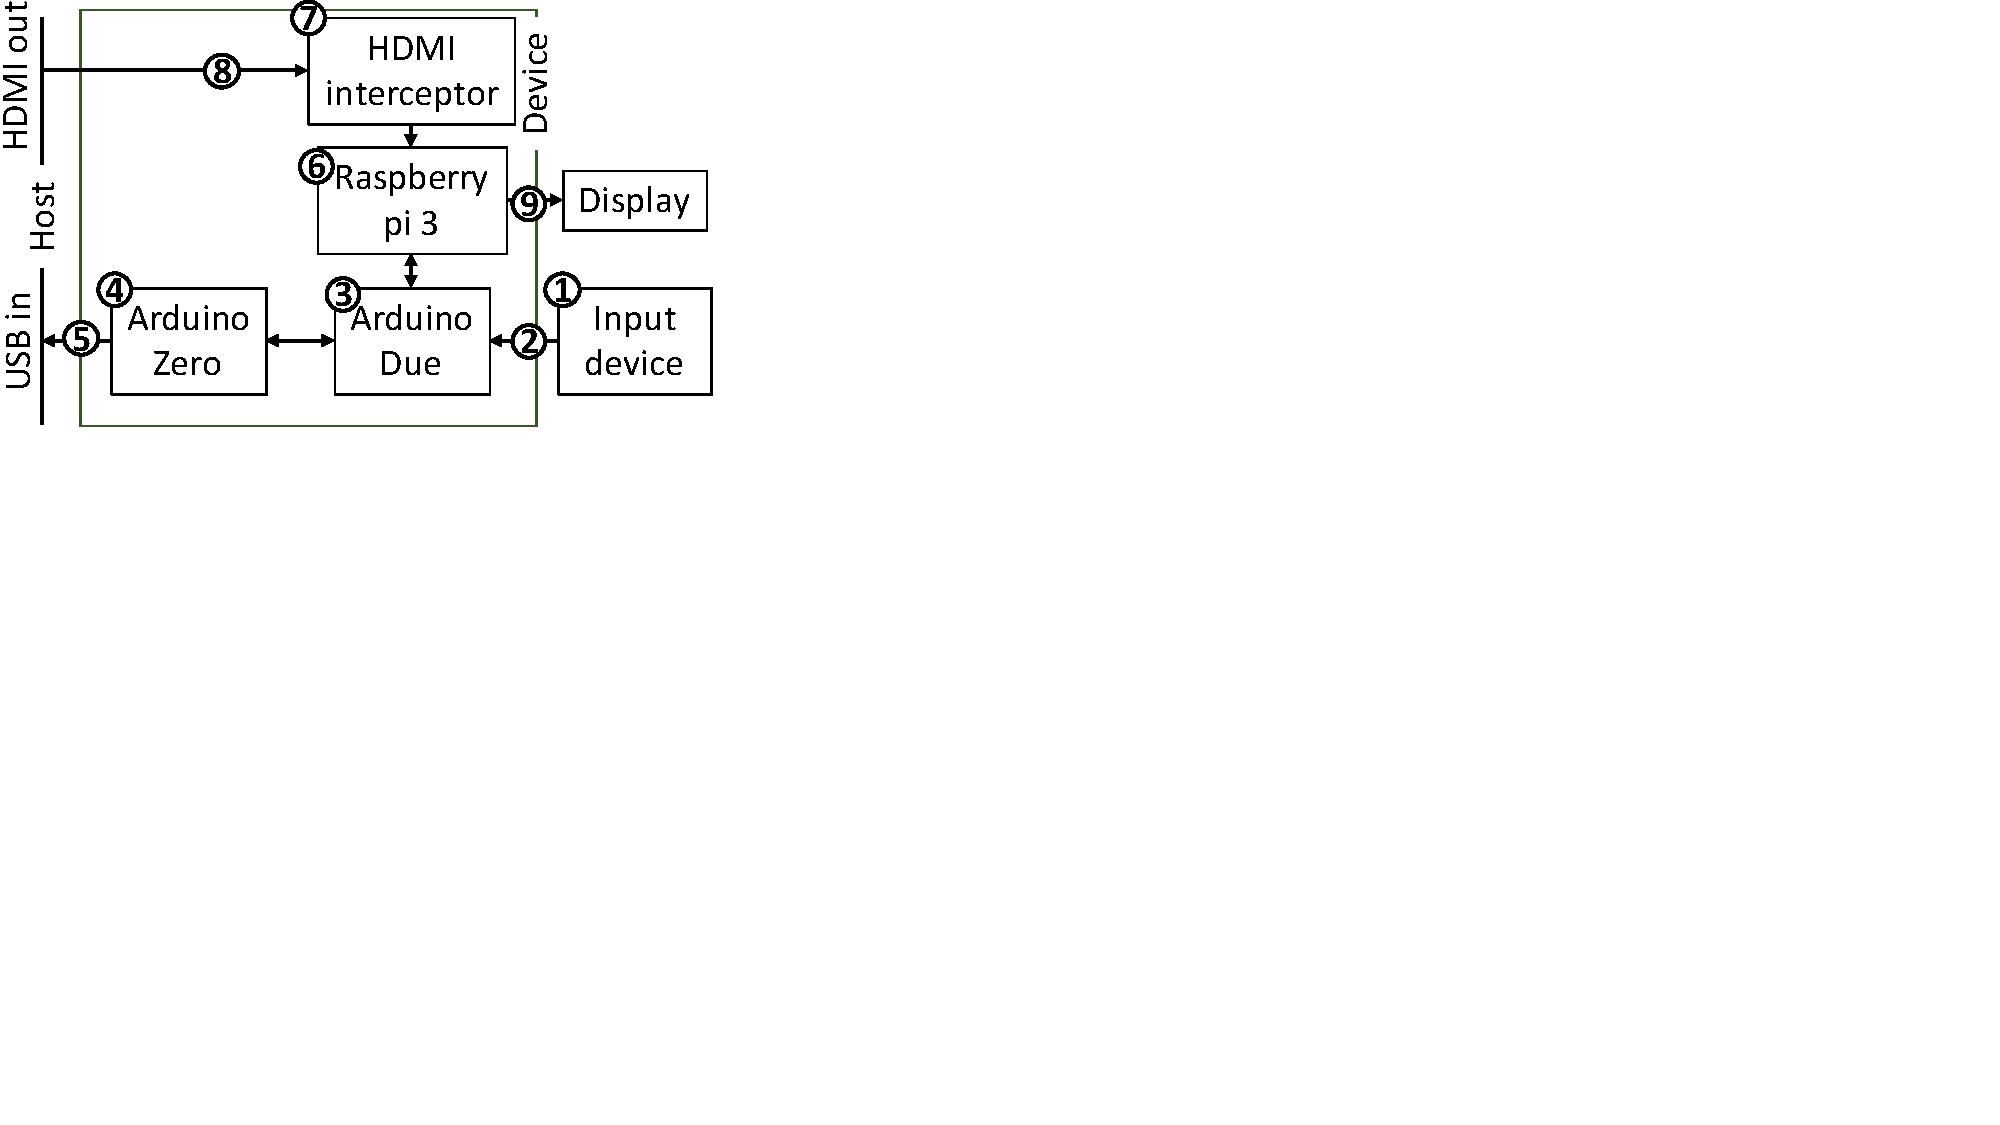
\includegraphics[trim={0 12cm 21.7cm 0}, clip, scale=0.45]{setUpBlock.pdf}
            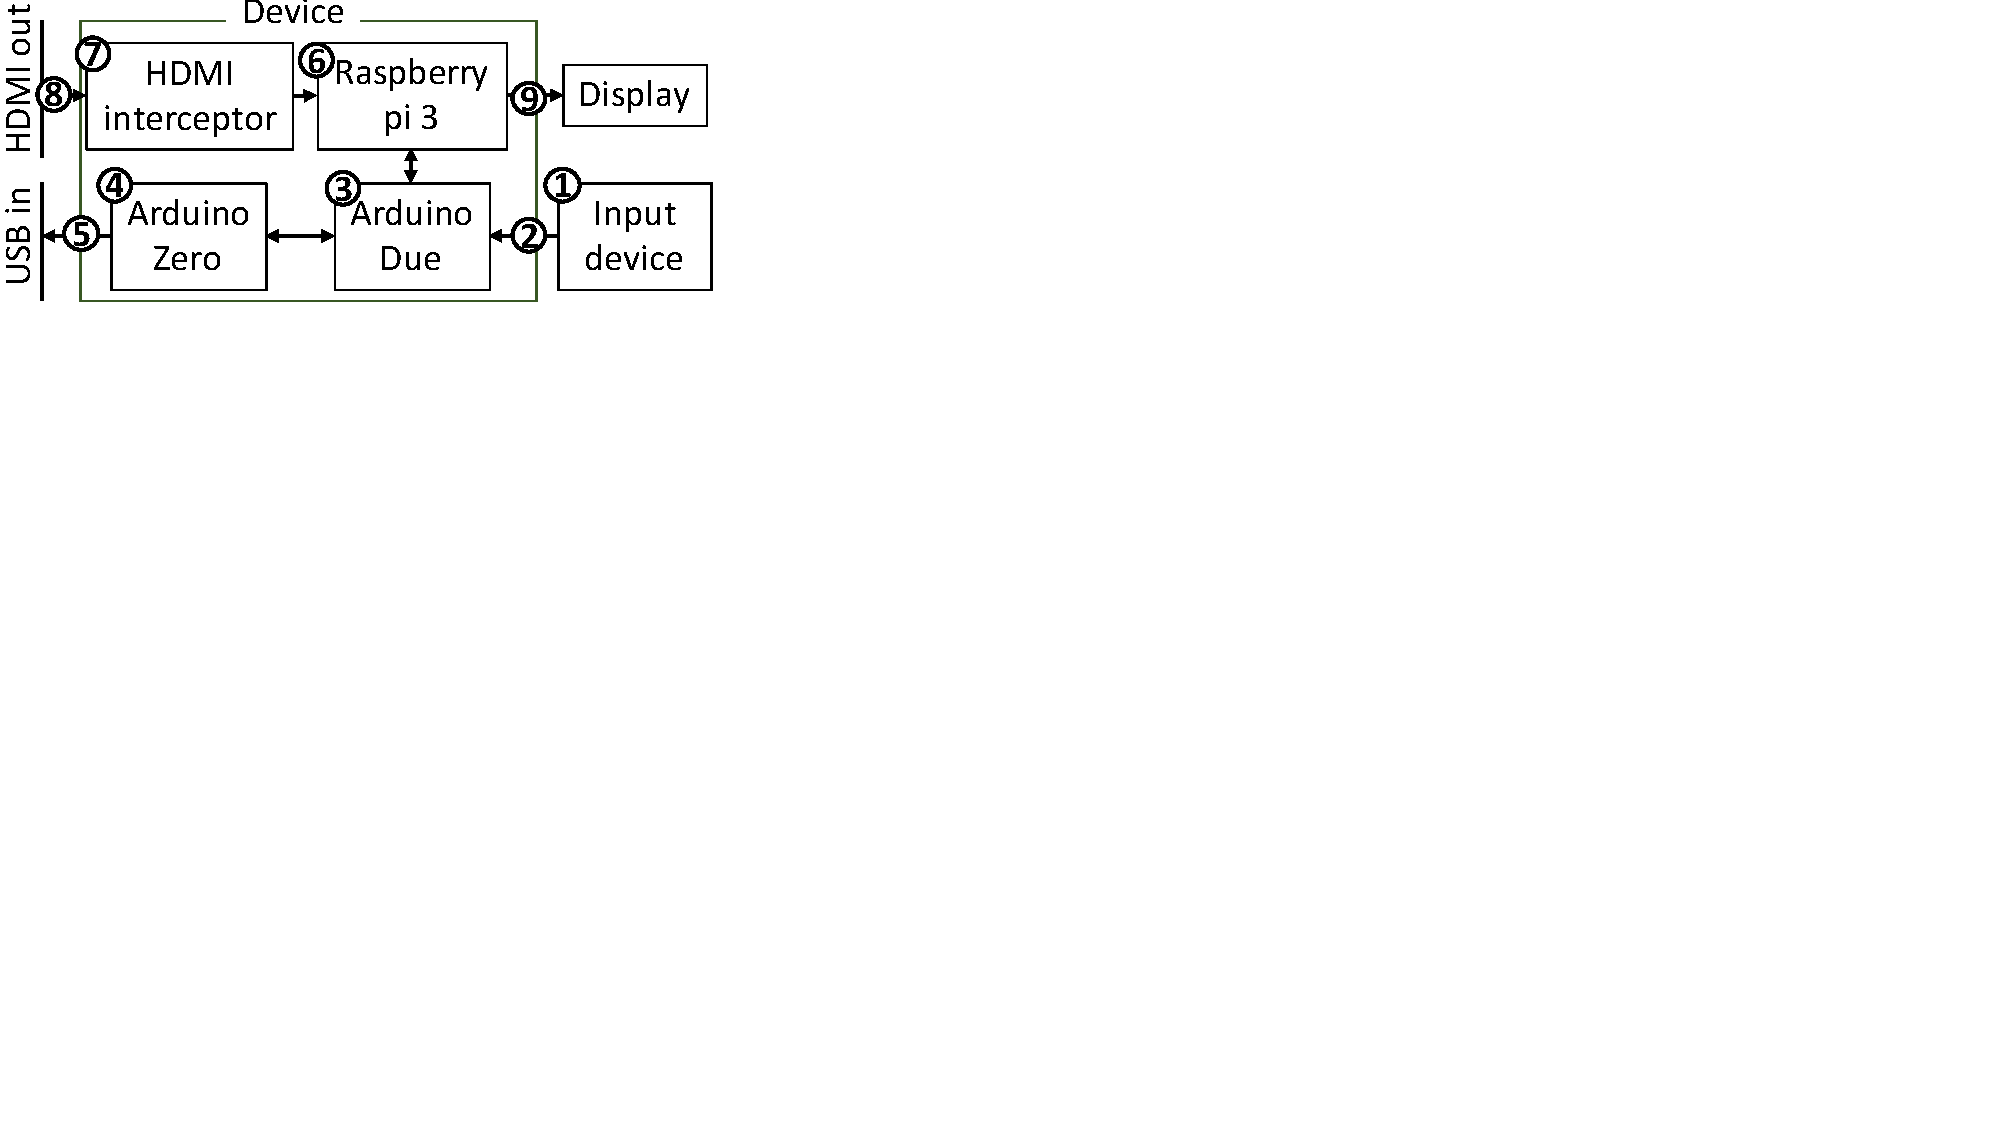
\includegraphics[trim={0 13.7cm 21.7cm 0}, clip, scale=0.4]{setUpBlock_1.pdf}
            \caption{The figure shows the basic components and connections between them in our \name prototype.}
            \label{fig:prototypeArch}    
        \end{subfigure}
    \end{center}
    
    %\vspace{1em} 
    
    \begin{center}
        \begin{subfigure}{0.4\textwidth}
        \centering
        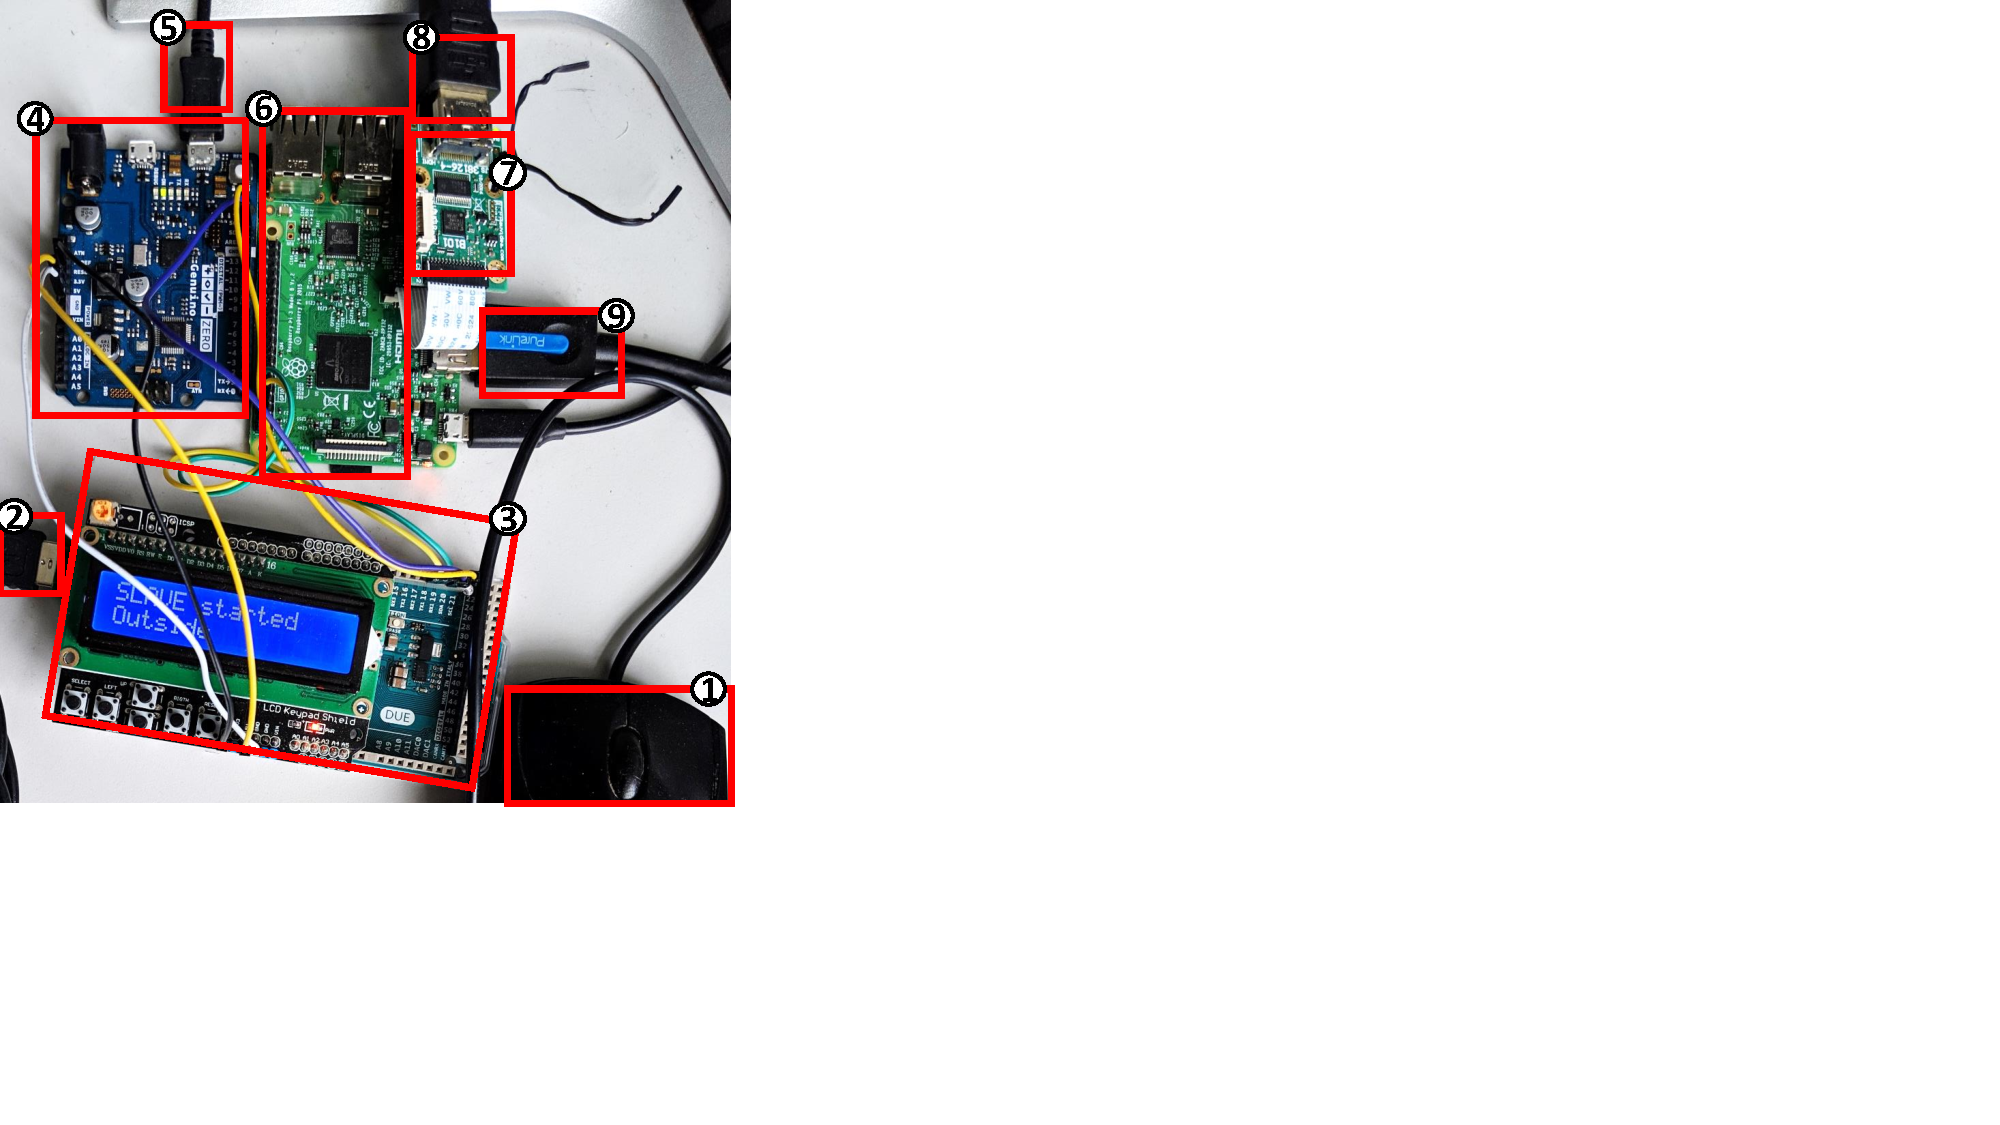
\includegraphics[trim={0 6.6cm 21.5cm 0}, clip, scale=0.5]{setUp_1.pdf}
        \caption{\name prototype uses Arduino Due and Zero microcontroller board and a Raspberry Pi 4 SBC. The highlighted numbers correspond to the labels in Figure~\ref{fig:prototypeArch}.}
        \label{fig:prototype}
    \end{subfigure}
    \end{center}
    \vspace{-1em}
    
    \caption{\textbf{\name prototype}. Figure~\ref{fig:prototypeArch} and~\ref{fig:prototype} shows the schematic and a photo of the  \name prototype respectively.} 
    \label{fig:prototypeAll}
    \spacesave
\end{figure}

\myparagraph{Setup} Here, we describe our prototype implementation of \name as an auxiliary device. Figure~\ref{fig:prototypeAll} depicts the \name prototype in two parts: Figure~\ref{fig:prototypeArch} shows the block diagram of our prototype with various components and connections, and Figure~\ref{fig:prototype} shows a photo of the actual prototype that highlights all the components described in the block diagram. The prototype \device is connected to a desktop computer with 3.40 GHz Intel Core i7-6700 processor with 8 GB RAM running Ubuntu 18.04.2 LTS. The \device uses off-the-shelf devices and has the following components (we use the same numbering as shown in Figure~\ref{fig:prototypeArch} and  Figure~\ref{fig:prototype}):

\begin{mylist}
 
  \item \textbf{Computing component.} We use a Raspberry Pi 4 (\six) to implement the computing component that executes all the \device logic that includes analyzing the HDMI frames, rendering the overlays, executing the \tls protocol, etc. One could use an ASIC to further improve the performance and reduce the code base of the component. The Pi is connected to the display over HDMI (\nine) interface. The code base of the Pi primarily consists of Python and Java.
  
  \item \textbf{Input interceptor.} The input interceptor is composed of an Arduino Due (\three) and an Arduino Zero (\four) that is connected to the input device over \usb (\two) interface. The input interceptor has a \usb out interface that connects to the host (\five) that relays all the user inputs to the host. 

  \item \textbf{HDMI interceptor.} The HDMI interceptor (\seven) is implemented using a B101 HDMI to CSI-2 Bridge~\cite{b101} that takes the HDMI channel (\eight) from the host and convert it to the camera input signal to the Raspberry Pi 4.  
 
\end{mylist}


